\section{\large \bf Introduction}

I am a second year student in the PhD in Engineering \– Concentration in Security program. The reason for taking this CS6000 course is that it is part of the requirements before one can become a candidate and hopefully go on to write a dissertation then defend it to successfully complete a PhD.

I work full time as a Security Systems Manager for Microsoft at the headquarters in Redmond, Washington. I have been with the company for approximately a year and a half. Microsoft has always been my dream company so I am very excited to be a part of it.

I got both my undergraduate (BS Computer Science and Systems) and graduate (Master of Cybersecurity and Leadership) degrees from the University of Washington – Tacoma in 2017 and 2018 respectively. Prior to getting into security, I started as a Software Developer.

\begin{figure}
  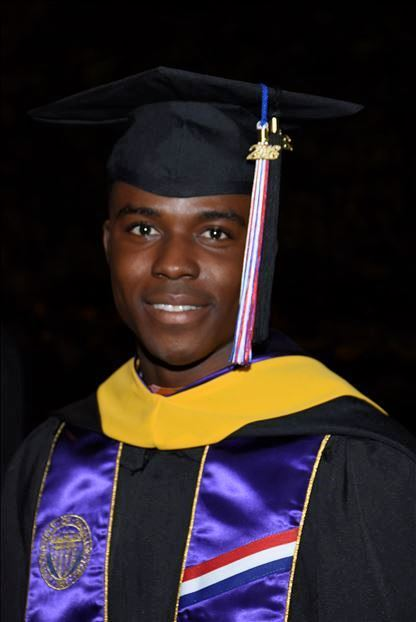
\includegraphics[width=\linewidth]{jbako.jpg}
  \caption{Picture of the Author (John Bako's graduation picture from Summer 2018)}
\end{figure}

\\
Question 1 by Parth: How did your career transition happen from software development to security? \\ 